\documentclass[12pt,letterpaper]{article}
\usepackage{graphicx,textcomp}
\usepackage{natbib}
\usepackage{setspace}
\usepackage{fullpage}
\usepackage{color}
\usepackage[reqno]{amsmath}
\usepackage{amsthm}
\usepackage{fancyvrb}
\usepackage{amssymb,enumerate}
\usepackage[all]{xy}
\usepackage{endnotes}
\usepackage{lscape}
\newtheorem{com}{Comment}
\usepackage{float}
\usepackage{hyperref}
\newtheorem{lem} {Lemma}
\newtheorem{prop}{Proposition}
\newtheorem{thm}{Theorem}
\newtheorem{defn}{Definition}
\newtheorem{cor}{Corollary}
\newtheorem{obs}{Observation}
\usepackage[compact]{titlesec}
\usepackage{dcolumn}
\usepackage{tikz}
\usetikzlibrary{arrows}
\usepackage{multirow}
\usepackage{xcolor}
\newcolumntype{.}{D{.}{.}{-1}}
\newcolumntype{d}[1]{D{.}{.}{#1}}
\definecolor{light-gray}{gray}{0.65}
\usepackage{url}
\usepackage{listings}
\usepackage{color}

\definecolor{codegreen}{rgb}{0,0.6,0}
\definecolor{codegray}{rgb}{0.5,0.5,0.5}
\definecolor{codepurple}{rgb}{0.58,0,0.82}
\definecolor{backcolour}{rgb}{0.95,0.95,0.92}

\lstdefinestyle{mystyle}{
	backgroundcolor=\color{backcolour},   
	commentstyle=\color{codegreen},
	keywordstyle=\color{magenta},
	numberstyle=\tiny\color{codegray},
	stringstyle=\color{codepurple},
	basicstyle=\footnotesize,
	breakatwhitespace=false,         
	breaklines=true,                 
	captionpos=b,                    
	keepspaces=true,                 
	numbers=left,                    
	numbersep=5pt,                  
	showspaces=false,                
	showstringspaces=false,
	showtabs=false,                  
	tabsize=2
}
\lstset{style=mystyle}
\newcommand{\Sref}[1]{Section~\ref{#1}}
\newtheorem{hyp}{Hypothesis}

\title{Replication - Agricultural idle time and armed conflict}
\date{Due: March 31, 2024}
\author{Applied Stats II}


\begin{document}
	\maketitle
	\section*{Introduction}
The aim of this project is to replicate the main figures and tables of the main findings found in the manuscript. Understand the method and approach used in the research and re-analyse the study using the knowledge gained from Stats I and Stats II with the aim to make a contribution.  

The scope of this project is on files: "Readme.txt" the instructions for a replication success, "DHR 2023 replicationA.do" the code used to create the main tables and figures, and ALLDataMerged 15May2023 weigted.dta  the dataset that serves as repository because contains the SCAD, ACLED and UCDP-GED datasets combined. 

In the next sessions you will find a brief explanation of the journal, the steps in the process of replication, and you also going to find the code in R and Stata to produce the main tables. 	
	\section*{Research Question}
The study aims to investigate the relationship between agricultural idle time and armed conflict in African countries.

	\section*{Theoretical Hypothesis}
Higher levels of agricultural idle time will be positively associated with the likelihood of observing armed conflict events.

	\vspace{.25cm}
\section*{Data Collection}
The academic paper of Agricultural idle time and armed conflict and its replication files can be found in Harvard Dataverse.
Here there is a list of the files found it and the possible outcome of each of them:
\vspace{.25cm}
\begin{itemize}
\item Africa admin1.dbf: This is a dBASE Table file for an ESRI Shapefile. Shapefiles are a common format used in geographic information systems (GIS) for storing geospatial vector data.
\item Africa admin1.shp: This file contains the main geometry data in ESRI Shapefile format. It likely represents administrative boundaries or other geographical features relevant to the study.
\item Africa admin1.shx: This file contains the shape index data for the ESRI Shapefile. It helps link the geometry information in the .shp file to attribute data in the .dbf file.
\item AllDataMerged 15May2023 weighted.dta: This is a Stata binary file (.dta) containing merged data used in the analysis. It seems to be the primary dataset for the study.
\item btscs-a-binary-time STATA.pdf: This PDF file might contain additional information, such as the methodology, results, or supplementary analyses conducted in Stata.
\item btscs.rar: This is a compressed archive file (.rar) that likely contains additional Stata do-files or other supplementary materials related to the analysis.
\item DHR 2023 LogFile.smcl: This file is written in Stata Markup and Control Language (SMCL) and may contain log output from the Stata analyses conducted for the paper.
\item DHR 2023 replicationA.do: This is a Stata do-file (.do) containing replication code or commands used for one part of the analysis.
\item DHR 2023 replicationB Map.do: Another Stata do-file (.do) containing replication code or commands, possibly related to mapping or visualizations.
\item ReadMe.txt: This plain text file likely contains instructions, explanations, or metadata related to the data and supplementary files.
\end{itemize}

\noindent Summary of Datasets Used:
\begin{itemize}
\item The Social Conflict Analysis Database (SCAD) includes protests, riots, strikes, inter-communal conflict, government violence against civilians, and other forms of social conflict not systematically tracked in other conflict datasets.
\item The Armed Conflict Location and Event Data Project (ACLED) collects real-time data on the locations, dates, actors, fatalities, and types of all reported political violence and protest events around the world.
\item Uppsala Conflict Data Program-Georeferenced Event Dataset (UCDP-GED) is the world’s main provider of data on organized violence and the oldest ongoing data collection project for civil war, with a history of almost 40 years. Its definition of armed conflict has become the global standard of how conflicts are systematically defined and studied.
\item Crop Location Data
\item Crop Calendar Charts
\end{itemize}




\newpage
\section*{Loading and Preprocessing the Data}
Due to the lack of information in the dataset I had to navigate into the data and get familiar with it. 
	
\begin{lstlisting}	

# load data
data <- read_dta("C:/Users/Antonio Felix/Dropbox/My PC (SHAW-72)/Downloads/AllDataMerged_15May2023_weighted.dta")

# Check the structure of the dataset
str(data)

# Getting familiar with the data
View(data)

# Understand the type of variables I have
head(data)

# Summarize the data
summary(data)
	
\end{lstlisting}	
	
	
\begin{verbatim}

tibble [277,872 × 210] (S3: tbl_df/tbl/data.frame)
 $ objectid                    : num [1:277872] 65 65 65 65 65 65 65 65 65 65 ...
..- attr(*, "label")= chr "OBJECTID"
..- attr(*, "format.stata")= chr "%8.0g"
$ month                       : chr [1:277872] "Jan" "Feb" "Mar" "Apr" ...
..- attr(*, "format.stata")= chr "%9s"
$ time_month                  : chr [1:277872] "Jan 1990" "Feb 1990" "Mar 1990" 


 objectid month time_month name_0  name_1 shape_area ISOcode country cultivated
<dbl> <chr> <chr>      <chr>   <chr>       <dbl> <chr>   <chr>        <dbl>
1       65 Jan   Jan 1990   Algeria Aïn …      0.456 DZA     Algeria       81.7
2       65 Feb   Feb 1990   Algeria Aïn …      0.456 DZA     Algeria       81.7
3       65 Mar   Mar 1990   Algeria Aïn …      0.456 DZA     Algeria       81.7
4       65 Apr   Apr 1990   Algeria Aïn …      0.456 DZA     Algeria       81.7
5       65 May   May 1990   Algeria Aïn …      0.456 DZA     Algeria       81.7
6       65 Jun   Jun 1990   Algeria Aïn …      0.456 DZA     Algeria       81.7
# 201 more variables: n_etype1 <dbl>, n_etype2 <dbl>, n_etype3 <dbl>,

> summary(data)
objectid       month            time_month           name_0         
Min.   :  65   Length:277872      Length:277872      Length:277872     
1st Qu.: 670   Class :character   Class :character   Class :character  
Median :1604   Mode  :character   Mode  :character   Mode  :character  
Mean   :1686                                                           
name_1            shape_area         ISOcode            country         
Length:277872      Min.   : 0.00009   Length:277872      Length:277872     
Class :character   1st Qu.: 0.20524   Class :character   Class :character  
Mode  :character   Median : 0.94572   Mode  :character   Mode  :character  
Mean   : 3.06470                             
\end{verbatim}	

Here we start to rename the variables, generate new ones, and replace values.

\begin{lstlisting}
STATA	
gen idle_index = IDLE_index
gen ym = date_month
lab var idle_index "Idle Index"

R STUDIO
# Rename variables
data$idle_index <- data$IDLE_index
data$ym <- data$date_month
names(data)[names(data) == "idle_index"] <- "Idle Index"

STATA
// set panel structure
xtset objectid ym

R STUDIO
# Set panel structure
library(plm)
pdata <- pdata.frame(data, index = c("objectid", "ym"))

STATA
gen SCADantigov = 0
replace SCADantigov = 1 if n_etype8 > 0 | n_etype9 > 0 
replace SCADantigov = . if n_etype8 == .

R STUDIO
# Generate variable and replace values
data$SCADantigov <- 0
data$SCADantigov[data$n_etype8 > 0 | data$n_etype9 > 0] <- 1
data$SCADantigov[is.na(data$n_etype8)] <- NA

STATA
gen py2  = py_SCADantigov * py_SCADantigov
gen py3  = py_SCADantigov * py_SCADantigov * py_SCADantigov

R STUDIO
# Generate squared and cubed variables
data$py2 <- data$py_SCADantigov^2
data$py3 <- data$py_SCADantigov^3

\end{lstlisting}

Generate Figure 1. Distribution of idle index

\begin{lstlisting}
STATA
reghdfe SCADantigov idle_index , absorb(objectid ) vce(r)  
gen sample = 1 if e(sample)==1

hist idle_index if sample==1 , scheme(s1mono)  percent ytitle(% of Observations) color(green%60) name(hist, replace) bin(20)
//graph export "Idlehist.pdf", replace

tabstat idle_index if sample==1 , by(mon)
graph bar (mean) idle_index if sample==1, over(Month, ) bar(1, fcolor(navy%60)) scheme(s1mono) ytitle(Mean Idle Index)  title(Mean by Month, size(medium)) name(meanovermon, replace)
///scatter cultivated idle_index if sample==1 , ytitle("% of cultivated land") scheme(s1mono) name(cult, replace) msymbol(oh) mcolor(red%30)

graph combine hist meanovermon, scheme(s1mono)
graph export "FigTbl/Fig1_Idlediag.pdf", replace

R STUDIO
# Load the necessary library
library(fixest)

# Load the dataset
data <- read.csv("AllDataMerged_15May2023_weighted.csv")

# Rename variables
data$idle_index <- data$IDLE_index
data$ym <- data$date_month

# Set panel structure
data <- pdata.frame(data, index = c("objectid", "ym"))

# Generate SCADantigov variable
data$SCADantigov <- ifelse(data$n_etype8 > 0 | data$n_etype9 > 0, 1, 0)
data$SCADantigov[data$n_etype8 == .] <- NA

# Run the fixed effects regression
model <- feols(SCADantigov ~ idle_index | objectid, data = data)

# Generate a sample indicator based on residuals
data$sample <- ifelse(!is.na(model$residuals), 1, 0)

# Subset data for the sample
sample_data <- subset(data, sample == 1)

# Histogram of idle_index
hist(sample_data$idle_index, main = "Distribution of Idle Index",
xlab = "Idle Index", ylab = "% of Observations", percent = TRUE, col = "green60", breaks = 20)

# Summary statistics by month
by_month <- tapply(sample_data$idle_index, sample_data$mon, summary)

# Bar plot of mean idle_index by month
barplot(by_month$mean, names.arg = names(by_month), xlab = "Month", ylab = "Mean Idle Index",
col = "navy60", main = "Mean by Month", border = NA)

# Export the graph
pdf("FigTbl/Fig1_Idlediag.pdf")
par(mfrow = c(1, 2))
hist(sample_data$idle_index, main = "Distribution of Idle Index",
xlab = "Idle Index", ylab = "% of Observations", percent = TRUE, col = "green60", breaks = 20)
barplot(by_month$mean, names.arg = names(by_month), xlab = "Month", ylab = "Mean Idle Index",
col = "navy60", main = "Mean by Month", border = NA)
dev.off()
\end{lstlisting}

R STUDIO
\begin{lstlisting}
# Load required libraries
library(ggplot2)
library(cowplot)

# Display the first few rows of data
head(data)

# Display the first few rows of monthly_mean_idle_index
head(monthly_mean_idle_index)

# Plotting Figure 1 again
# Distribution of idle index (left panel)
histogram <- ggplot(data = data, aes(x = IDLE_index)) +
geom_histogram(binwidth = 0.005, fill = "red", color = "red", alpha = 0.8) +  # Set both fill and color to "red"
labs(title = "Distribution of Idle Index",
x = "Idle Index",
y = "Frequency") +
theme_minimal()

# Mean of idle index for each month across Africa (right panel)
lineplot <- ggplot(data = monthly_mean_idle_index, aes(x = month, y = monthly_mean_idle_index)) +
geom_line(color = "blue", size = 1) +  # Use geom_line() for a line plot
labs(title = "Mean Idle Index for Each Month",
x = "Month",
y = "Mean Idle Index") +
theme_minimal() +
theme(axis.text.x = element_text(angle = 45, hjust = 1))  # Rotate x-axis labels for better readability

# Combine both plots
combined_plot <- cowplot::plot_grid(histogram, lineplot, labels = "AUTO", nrow = 1)

# Display the combined plot
print(combined_plot)		
\end{lstlisting}

\begin{figure}[htbp]
	\centering
	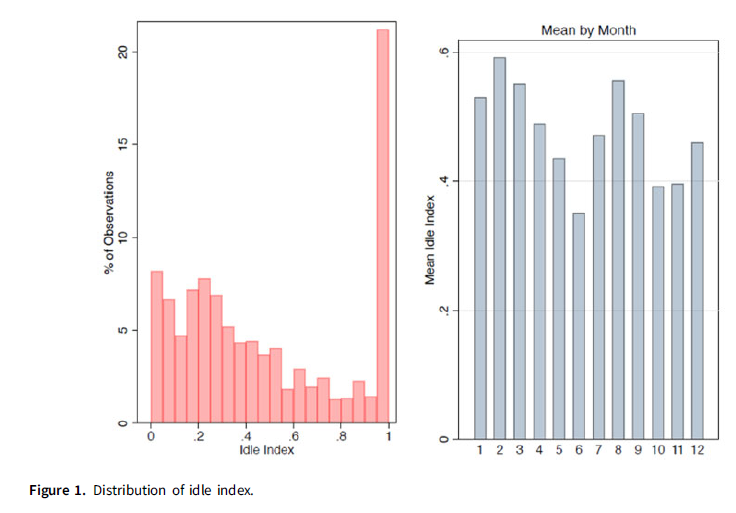
\includegraphics[width=1.0\textwidth]{Figure 1 Distribution of idle index.png}
	\caption{Distribution of idle index}
	\label{fig:agri_conflict}
\end{figure}


Generate Table 1: Agricultural idle time and armed conflict

\begin{lstlisting}

STATA	
			
** SCAD analysis:

egen yearmon = group(year mon) 
egen oyfe = group(objectid year)
// gen object year FE

//gen lnpy_SCAD = ln(py_SCADantigov+.1)

est clear 
sum SCADantigov if sample==1 
local bl = r(mean) 

eststo: reghdfe SCADantigov idle_index , absorb(objectid ) vce(r)  
estadd local FEobj"x"
estadd local perch =  (_b[idle_index]/`bl')*100
di  ((_b[idle_index]*.35)/`bl')*100
//estadd local perch50 =  ((_b[idle_index]*.63)/`bl')*100

*eststo: reghdfe SCADantigov idle_index , absorb(ccode) vce(r)  
*estadd local FEcountry"x"
*estadd local perch =  (_b[idle_index]/`bl')*100

eststo: reghdfe SCADantigov idle_index , absorb(oyfe ) vce(r)  
estadd local FEoy "x"
estadd local perch =  (_b[idle_index]/`bl')*100

eststo: reghdfe SCADantigov idle_index , absorb(objectid oyfe) vce(r )  
estadd local FEobj"x"
estadd local FEoy "x"
estadd local perch =  (_b[idle_index]/`bl')*100

eststo: reghdfe SCADantigov idle_index , absorb(objectid oyfe ym ) vce(r )  
estadd local FEobj"x"
estadd local FEoy "x"
estadd local FEmo "x"
estadd local perch =  (_b[idle_index]/`bl')*100

eststo: reghdfe SCADantigov idle_index temp prec, absorb(objectid oyfe mon ) vce(r)  
estadd local FEobj"x"
estadd local FEoy "x"
estadd local FEmo "x"
estadd local TP "x"
estadd local perch =  (_b[idle_index]/`bl')*100

eststo: reghdfe SCADantigov idle_index py_SCADantigov, absorb(objectid oyfe mon ) vce(r)  
estadd local FEobj"x"
estadd local FEoy "x"
estadd local FEmo "x"
estadd local PY "x"
estadd local perch =  (_b[idle_index]/`bl')*100

#delimit ; 
esttab _all using "FigTbl/Table1_SCAD.csv", label nogaps compress 
keep(idle_index)  se star(* 0.05 ** 0.01 *** 0.001) cells(b(star fmt(%9.4f)) se( fmt(%9.4f)))
stats(perch N r2 FEobj FEoy FEcountry FEmo TP PY, fmt(%2.1f %18.0g %12.2f) labels(`"Per. Change"' `"Observations"' `"R-squared"' `"Location FE"' `"Country-Year FE"' `"Country FE"' `"Calendar Month FE"' `"Temp & Precipitation"' `"Peace Months"') )
replace ; 
#delimit cr 


** ACLED initiator ***

est clear 

*gen acled_bi = (ACLED_initiator_count>0)
*replace acled_bi = . if ACLED_initiator_count==.

btscs acled_bi year objectid, g(py_acled_bi)

gen py2_acled  = py_acled_bi*py_acled_bi
gen py3_acled  = py_acled_bi*py_acled_bi*py_acled_bi


sum acled_bi if sample==1 
local bl = r(mean) 

est clear
eststo: reghdfe acled_bi idle_index , absorb(objectid ) vce(r)  
estadd local FEobj"x"
estadd local perch =  (_b[idle_index]/`bl')*100

eststo: reghdfe acled_bi idle_index , absorb( oyfe) vce(r )  
estadd local FEoy "x"
estadd local perch =  (_b[idle_index]/`bl')*100

eststo: reghdfe acled_bi idle_index , absorb(objectid oyfe) vce(r )  
estadd local FEobj"x"
estadd local FEoy "x"
estadd local perch =  (_b[idle_index]/`bl')*100

eststo: reghdfe acled_bi idle_index , absorb(objectid oyfe mon ) vce(r )  
estadd local FEobj"x"
estadd local FEoy "x"
estadd local FEmo "x"
estadd local perch =  (_b[idle_index]/`bl')*100

eststo: reghdfe acled_bi idle_index temp prec, absorb(objectid oyfe mon ) vce(r)  
estadd local FEobj"x"
estadd local FEoy "x"
estadd local FEmo "x"
estadd local TP "x"
estadd local perch =  (_b[idle_index]/`bl')*100

eststo: reghdfe acled_bi idle_index py_acled_bi, absorb(objectid oyfe mon ) vce(r)  
estadd local FEobj"x"
estadd local FEoy "x"
estadd local FEmo "x"
estadd local PY "x"
estadd local perch =  (_b[idle_index]/`bl')*100

#delimit ; 
esttab _all using "FigTbl/Table1_ACLED.csv", label nogaps compress 
keep(idle_index)  se star(* 0.05 ** 0.01 *** 0.001) 
stats(perch N r2 FEobj FEoy FEmo TP PY, fmt(%3.2f %18.0g %12.2f) labels(`"Per. Change"' `"Observations"' `"R-squared"' `"Location FE"' `"Location-Year FE"' `"Calendar Month FE"' `"Temp & Precipitation"' `"Peace Months"') )
replace ; 
#delimit cr 


** UCDP ***

*gen UCDP_bi = (UCDP_Violent_init_count>0)
*replace UCDP_bi = . if UCDP_Violent_init_count==.

reghdfe UCDP_bi idle_index , absorb(objectid ) vce(r)  
gen sample_ucdp =1 if e(sample)==1

btscs UCDP_bi year objectid, g(py_UCDP_bi)

gen py2_ucdp  = py_UCDP_bi*py_UCDP_bi
gen py3_ucdp  = py_UCDP_bi*py_UCDP_bi*py_UCDP_bi


est clear 
sum UCDP_bi if sample_ucdp==1 
local bl = r(mean) 

est clear
eststo: reghdfe UCDP_bi idle_index , absorb(objectid ) vce(r)  
estadd local FEobj"x"
estadd local perch =  (_b[idle_index]/`bl')*100

eststo: reghdfe UCDP_bi idle_index , absorb( oyfe) vce(r )  
estadd local FEoy "x"
estadd local perch =  (_b[idle_index]/`bl')*100

eststo: reghdfe UCDP_bi idle_index , absorb(objectid oyfe) vce(r )  
estadd local FEobj"x"
estadd local FEoy "x"
estadd local perch =  (_b[idle_index]/`bl')*100

eststo: reghdfe UCDP_bi idle_index , absorb(objectid oyfe mon ) vce(r )  
estadd local FEobj"x"
estadd local FEoy "x"
estadd local FEmo "x"
estadd local perch =  (_b[idle_index]/`bl')*100

eststo: reghdfe UCDP_bi idle_index temp prec, absorb(objectid oyfe mon ) vce(r)  
estadd local FEobj"x"
estadd local FEoy "x"
estadd local FEmo "x"
estadd local TP "x"
estadd local perch =  (_b[idle_index]/`bl')*100

eststo: reghdfe UCDP_bi idle_index py_UCDP_bi, absorb(objectid oyfe mon ) vce(r)  
estadd local FEobj"x"
estadd local FEoy "x"
estadd local FEmo "x"
estadd local PY "x"
estadd local perch =  (_b[idle_index]/`bl')*100

#delimit ; 
esttab _all using "FigTbl/Table1_UCDP.csv", label nogaps compress 
keep(idle_index)  se star(* 0.05 ** 0.01 *** 0.001) 
stats(perch N r2 FEobj FEoy FEmo TP PY, fmt(%3.2f %18.0g %12.2f) labels(`"Per. Change"' `"Observations"' `"R-squared"' `"Location FE"' `"Location-Year FE"' `"Calendar Month FE"' `"Temp & Precipitation"' `"Peace Months"') )
replace ; 
#delimit cr 

\end{lstlisting}

\newpage
STATA
\begin{figure}[htbp]
	\centering
	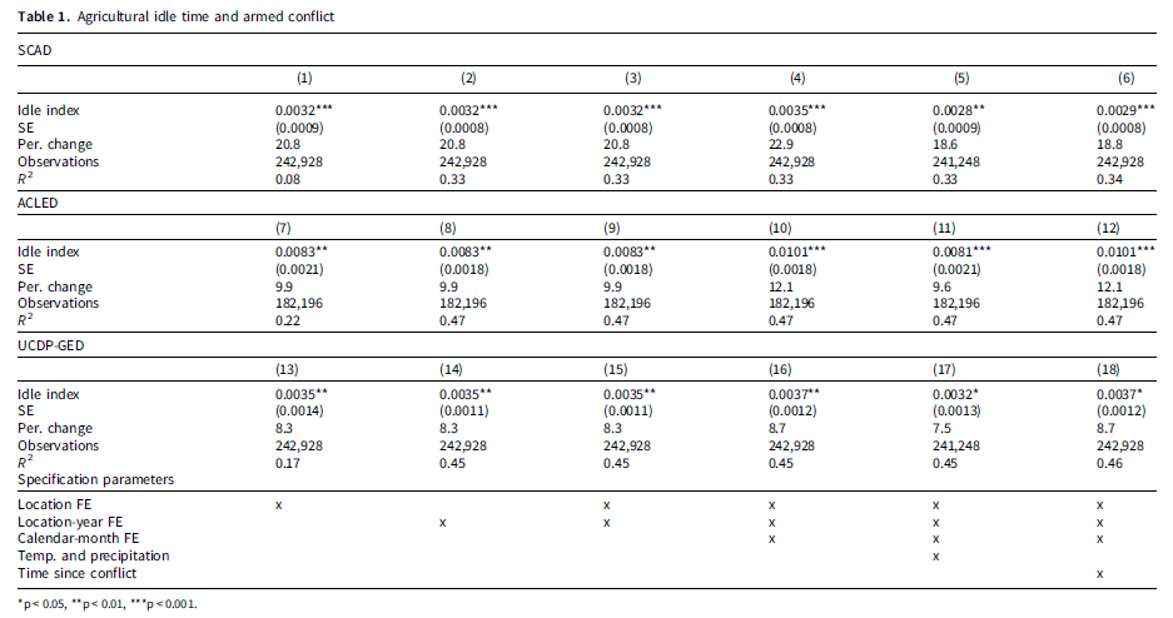
\includegraphics[width=1.0\textwidth]{Table 1 Agricultural idle time and armed conflict.png}
	\caption{Agricultural idle time and armed conflict}
	\label{fig:agri_conflict}
\end{figure}


\begin{verbatim}
R Studio	
Table 1 Agricultural idle time and armed conflict

	|Dataset  | Estimate|     SE| Perc Change| Observations|   R2|
	|:--------|--------:|------:|-----------:|------------:|----:|
	|SCAD     |   0.0032| 0.0009|        20.8|       242928| 0.08|
	|SCAD     |   0.0032| 0.0008|        20.8|       242928| 0.33|
	|SCAD     |   0.0032| 0.0008|        20.8|       242928| 0.33|
	|SCAD     |   0.0035| 0.0008|        22.9|       242928| 0.33|
	|SCAD     |   0.0028| 0.0009|        18.6|       241248| 0.33|
	|SCAD     |   0.0029| 0.0008|        18.8|       242928| 0.34|
	|ACLED    |   0.0083| 0.0021|         9.9|       182196| 0.22|
	|ACLED    |   0.0083| 0.0018|         9.9|       182196| 0.47|
	|ACLED    |   0.0083| 0.0018|         9.9|       182196| 0.47|
	|ACLED    |   0.0101| 0.0018|        12.1|       182196| 0.47|
	|ACLED    |   0.0081| 0.0021|         9.6|       182196| 0.47|
	|ACLED    |   0.0101| 0.0018|        12.1|       182196| 0.47|
	|UCDP-GED |   0.0035| 0.0014|         8.3|       242928| 0.17|
	|UCDP-GED |   0.0035| 0.0011|         8.3|       242928| 0.45|
	|UCDP-GED |   0.0035| 0.0011|         8.3|       242928| 0.45|
	|UCDP-GED |   0.0037| 0.0012|         8.7|       242928| 0.45|
	|UCDP-GED |   0.0032| 0.0013|         7.5|       241248| 0.45|
	|UCDP-GED |   0.0037| 0.0012|         8.7|       242928| 0.46|	
	
\end{verbatim}

Dependent Variables: Three different measures of conflict are used: SCAD (Social Conflict Analysis Database), ACLED (Armed Conflict Location Event Dataset), and UCDP-GED (Uppsala Conflict Data Program-Georeferenced Event Dataset). Each measure captures different aspects of political violence.

Independent Variable: The agricultural idle index is the main independent variable of interest. The coefficients indicate the change in the probability of conflict occurrence associated with a one-unit increase in the idle index.


The coefficients for the idle index are statistically significant across all specifications and outcome variables, indicated by the p-values (p < 0.01 or *p < 0.001).
The magnitude of the coefficients suggests that an increase in the agricultural idle index is associated with a significant increase in the probability of conflict occurrence. For example, in the SCAD model, a one-unit increase in the idle index is associated with a 20.8% increase in the probability of conflict.
The models' explanatory power, indicated by the R-squared values, varies across specifications but generally falls within the range of 0.08 to 0.47, suggesting moderate to substantial explanatory power.


\newpage

Generate Table 2: Idle index post-2000 - SCAD

\begin{lstlisting}
STATA
est clear 
sum SCADantigov  if sample==1 &  year>2000
local bl = r(mean) 

est clear
eststo: reghdfe SCADantigov idle_index if year>2000, absorb(objectid ) vce(r)  
estadd local FEobj"x"
estadd local perch =  (_b[idle_index]/`bl')*100

eststo: reghdfe SCADantigov idle_index  if year>2000, absorb( oyfe) vce(r )  
estadd local FEoy "x"
estadd local perch =  (_b[idle_index]/`bl')*100

eststo: reghdfe SCADantigov idle_index  if year>2000, absorb(objectid oyfe) vce(r )  
estadd local FEobj"x"
estadd local FEoy "x"
estadd local perch =  (_b[idle_index]/`bl')*100

eststo: reghdfe SCADantigov idle_index  if year>2000, absorb(objectid oyfe mon ) vce(r )  
estadd local FEobj"x"
estadd local FEoy "x"
estadd local FEmo "x"
estadd local perch =  (_b[idle_index]/`bl')*100

eststo: reghdfe SCADantigov idle_index temp prec  if year>2000, absorb(objectid oyfe mon ) vce(r)  
estadd local FEobj"x"
estadd local FEoy "x"
estadd local FEmo "x"
estadd local TP "x"
estadd local perch =  (_b[idle_index]/`bl')*100

eststo: reghdfe SCADantigov idle_index py_SCADantigov  if year>2000, absorb(objectid oyfe mon ) vce(r)  
estadd local FEobj"x"
estadd local FEoy "x"
estadd local FEmo "x"
estadd local PY "x"
estadd local perch =  (_b[idle_index]/`bl')*100

#delimit ; 
esttab _all using "FigTbl/Table2_POST2000.csv", label nogaps compress 
keep(idle_index)  se star(* 0.05 ** 0.01 *** 0.001)  cells(b(star fmt(%9.4f)) se( fmt(%9.4f)))
stats(perch N r2 FEobj FEoy FEmo TP PY, fmt(%3.2f %18.0g %12.2f) labels(`"Per. Change"' `"Observations"' `"R-squared"' `"Location FE"' `"Location-Year FE"' `"Calendar Month FE"' `"Temp & Precipitation"' `"Peace Months"') )
replace ; 
#delimit cr 
\end{lstlisting}

STATA
\begin{figure}[htbp]
	\centering
	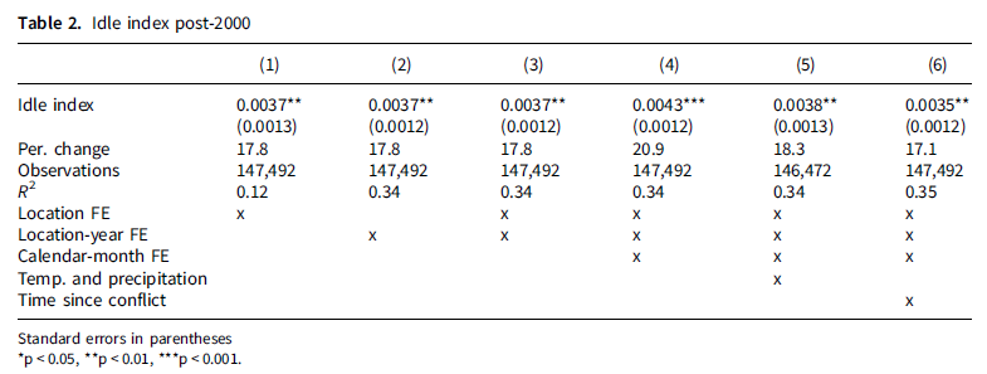
\includegraphics[width=1.0\textwidth]{Table 2 Idle index post-2000 - SCAD.png}
	\caption{Idle index post-2000 - SCAD}
	\label{fig:agri_conflict}
\end{figure}

R Studio

Table 2 Idle index post-2000 - SCAD
\begin{verbatim}
| Estimate|     SE| Perc Change| Observations|   R2|
|--------:|------:|-----------:|------------:|----:|
|   0.0037| 0.0013|        17.8|       147492| 0.12|
|   0.0037| 0.0012|        17.8|       147492| 0.34|
|   0.0037| 0.0012|        17.8|       147492| 0.34|
|   0.0043| 0.0012|        20.9|       147492| 0.34|
|   0.0038| 0.0013|        18.3|       146472| 0.34|
|   0.0035| 0.0012|        17.1|       147492| 0.35|
\end{verbatim}

The coefficients for the idle index remain statistically significant across all specifications and outcome variables, denoted by the significance levels (p < 0.01 or *p < 0.001).
Consistent with the findings from Table 1, the coefficients indicate a positive association between agricultural idle time and the likelihood of conflict occurrence. For instance, in the SCAD model, a one-unit increase in the idle index is associated with a 17.8 percentage increase in the probability of conflict.
The explanatory power of the models, as indicated by the R-squared values, remains moderate to substantial, ranging from 0.12 to 0.35.

Overall, the results from Table 2 reaffirm the positive association between agricultural idle time and conflict occurrence, even when focusing specifically on the post-2000 period

\newpage
\section*{Contribution}

Generate R Studio Code for replication of the main tables and figures. 

\section*{Conclusion}
About the dataset: 
Choosing a different academic paper where the code is already in R Studio, can avoid wasted time and allow us to focus on the paper's goal.
An explanation about the variables in the dataset is missing this potentially could help to improve the contribution on the study. 


\end{document}
